\documentclass[main.tex]{subfiles}
 
\begin{document}
%The electric grid 

%The thesis that you are currently reading

%Unless you are reading a handwritten copy of this thesis in your back yard, 

%{
%(100W = 16-candela = 200lm = 2.2Watt bij ikea)
%
%
%30\%? of energy use is transported using the grid
%
%list of synchronous grids
%
%complexity
%
%why interconnect? separate generation and load; economy of scale; security (distributed peak demand); stability; 
%
%}

\emph{This chapter is based on two books: \emph{Electric Power Systems} by \cite{VonMeier2006}, which provides a clear summary of the working and operation of electric grids, and \emph{Electric Power Principles: Sources, Conversion, Distribution and Use} by \cite{Kirtley2010}, a more quantitative approach to the subject.}
\section{Overview}
The electric grids of this world are some of the largest machines built by humans. As this system was built by clever engineers, its behaviour is, on a small scale (individual lines, transformers, and so on) \emph{well-understood}. In fact, one of the reasons that all transmission lines, substations and switchboxes look so similar, is to increase the \emph{homogeneity} of the network.

On a larger scale, however, the behaviour of this machine is not always well understood, as complex behaviour arises from the interconnection of generators, transmission lines and loads.
%The screen that you are reading this thesis on, or the printer that was used to print it, is most likely connected
When the transmission network fails, the consequences can be dramatic. For example, filtering and supply of drinking water, telecommunication and heating all rely on a functioning power grid. The large scale of a transmission network makes it more stable, but it also increases the potential effect of its failure. The two largest blackouts (at the time of writing) occurred in north-eastern India on 30 and 31 July, 2012, affecting 400 million and 620 million people, respectively. These blackouts were due to a peak in consumption caused by extreme heat and drought.\footnote{Air-conditioning and irrigation pumps increased consumption; hydroelectric generation was limited.}
\section{Generators}
Almost all sources of electric power in the electric grid use an \define{AC generator}\index{generator} to convert (rotational) kinetic energy to electric energy.\footnote{A notable exception is the photovoltaic cell (PV cell) used in solar panels. PV cells produce a direct current, which is converted to AC power at nominal voltage using an \define{inverter}. Solar inverters are often complicated systems, capable of using battery storage, synchronising with the AC grid and varying PV operating voltage to maximise PV efficiency.} 
At a hydroelectric plant, the weight of water applies direct torque to the water pumps, mechanically connected to the generator shaft.\footnote{Some hydroelectric plants are \emph{reversible}: their generators can be used as electric motors, pumping water back up into a reservoir. This is a form of large-scale \define{energy storage}, which can increase the usability of intermittent renewable energy sources.}
At most other types of plants (including coal-fired and nuclear plants), generators are powered by steam pressure. 

The term \define{AC generator} denotes a specific device that uses \emph{electromagnetic induction} to convert rotational kinetic energy into AC power. Somewhat confusingly, we use the term \define{generator} to denote \emph{any} energy source connected to the grid, where we consider a power plant (which might house multiple AC generators) as a single generator. Solar parks and lithium batteries are generators, but they do not use an AC generator. They use an AC inverter, which \emph{mimics}, to some extent, the behaviour of a classical AC generator.
 
\section{Loads}\label{sec:loads}
%\towrite{load profiling, load series, fridge duty cycle example, reactive load, power factor}
Unlike other utilities like gas and water, the transfer of electrical energy is \emph{instantaneous}.\footnote{Within the limits of special relativity, of course. That is, while the drift speed electrons is nowhere near the speed of light, the actual \emph{signal} propagates at about two thirds the speed of light, depending on the type of cable.} Of course, energy storage does exist,\footnote{Most commonly as \emph{reversible} hydro-electric generators; other examples include hydrogen storage (electrolysis of water produces hydrogen and oxygen, which can be stored and combusted at a later time) and lithium storage (very large phone batteries) (some electric vehicles can also return energy back to grid!)} but this energy is not stored as `high-voltage AC energy', but as \emph{potential} (mechanical or chemical) energy. Potential energy needs to be converted before it can be transmitted, which is not instantaneous. When switching on your lights, there will be an \emph{instant} increase in demand, which must be generated somewhere (otherwise it would violate the Law of Conservation of Energy). Of course, via the electric grid, your light bulb is connected to generators, which then start converting an additional $10 \, \si{\watt}$ to power the light bulb. But how do the generators know when to increase their output, if you never called them to say that you are turning on your lights? 

The answer is called \define{electric inertia}. A classic AC generator (in a hydroelectric plant, for example) contains a heavy rotor, which is spinning at (a rational fraction of) the grid frequency. Because of its weight, a lot of energy is stored in the spinning of the rotor. When the total load on an AC network is increased, there is no instantaneous increase in burning of fuel, flowing of water, or otherwise. Instead, this increase in power demand will `take' its energy from the \emph{inertial energy} of all rotational AC generators in the grid, \emph{slowing down} their rotation. As a result, the AC frequency of the entire grid starts slowing down. When grid operators notice a drop in AC frequency (we are talking about differences on the order of $0.001\,\si{\hertz}$ here), they can increase the amount of fuel being burned, open water valves or lift control rods from between radioactive cores to increase the amount of energy converted by the AC generator. This will start to increase the AC frequency again, until it settles at the predetermined utility frequency ($60\,\si{\hertz}$ in North America and Northern South America; $50\,\si{\hertz}$ in the rest of the world, with some exceptions).
Most modern AC generators have an automatic feedback loop to control the steam valve, to allow for frequency adjustments on the smallest scale.




\section{Transmission}
The voltage of AC power can be shifted up and down using transformers. We typically use higher voltages for long-range transmission, since high-voltage AC is much more efficient (less power is lost in heating the transmission lines). This is why high-voltage lines can afford to have relatively thin wires, given the amount of power that they transmit. The network of high-voltage lines (which operate at voltages on the order of $100 \, \si{\kilo\volt}$) is called the \emph{transmission network}. Transmission lines usually run interrupted for long distances (on the order of kilometres) between two \emph{substations}. At these endpoints, transformers connect the high-voltage transmission lines to medium-voltage (on the order of $10 \, \si{\kilo\volt}$) \emph{distribution lines}, which eventually make it to all generators and consumers in the area that the substation serves.

\subsection{Three-phase transmission}\label{sec:threephase}
Depending on where you live, your wall socket will likely have \emph{two} connectors. Most modern sockets also have a third connector, the \emph{ground wire}, but this third connector does not have the purpose of carrying a current, like the other two (under normal circumstances).

This makes sense, since most electrical devices only need a \emph{potential difference} (between \emph{two} wires) to function. In the early days of transmission systems, however, this caused a problem for factories using AC motors to power their production line. When a (single-phase) AC current is used to power a motor, the amount of \emph{torque}
\footnote{\ie rotational force. In most systems, torque is proportional to \emph{change in rotational velocity} (change in rpm).}
is not constant: when the potential difference is zero, which happens twice every $1/50^{\text{th}}$ of a second, no electric field is present in the armature windings, and no torque is applied to the rotor.

To solve this problem, both the AC generator and AC motor are equipped with \emph{three} identical sets of armature windings, each oriented $120 \si{\degree}$ relative to the others. One end of each winding is connected to the common ground, and the remaining three connection points form the \emph{three-phase connection} between generator and motor.\footnote{This method of connecting three coils (or more generally, impedances) to three-phase AC is called the \emph{Wye configuration}. Another method is to connect the impedances between each pair of two phases, with no common ground connection. This method, called the \emph{Delta} configuration, is described in more detail in \cite{VonMeier2006}.}

As the generator rotor is moving, there will always be one armature winding which is close \footnote{within $30 \si{\degree}$} to being perpendicular to the rotor windings, and will therefore have a relatively high induced current. 

In fact, when writing down the three currents in exact form (three sinusoids with the same frequency and magnitude, with phases $0\si{\degree}$, $120\si{\degree}$ and $240\si{\degree}$), we find that \emph{the sum of their squares}, \ie the total amount of transmitted power, \emph{is constant}! Although the amount of power transmitted on just one of the phases (square of the sinusoid current) is not constant, the combination of the three is. This means that the torque of a motor, which is the sum of torques applied by each armature winding, is constant.

\begin{figure}[ht]
\begin{subfigure}{\textwidth}
    \centering
    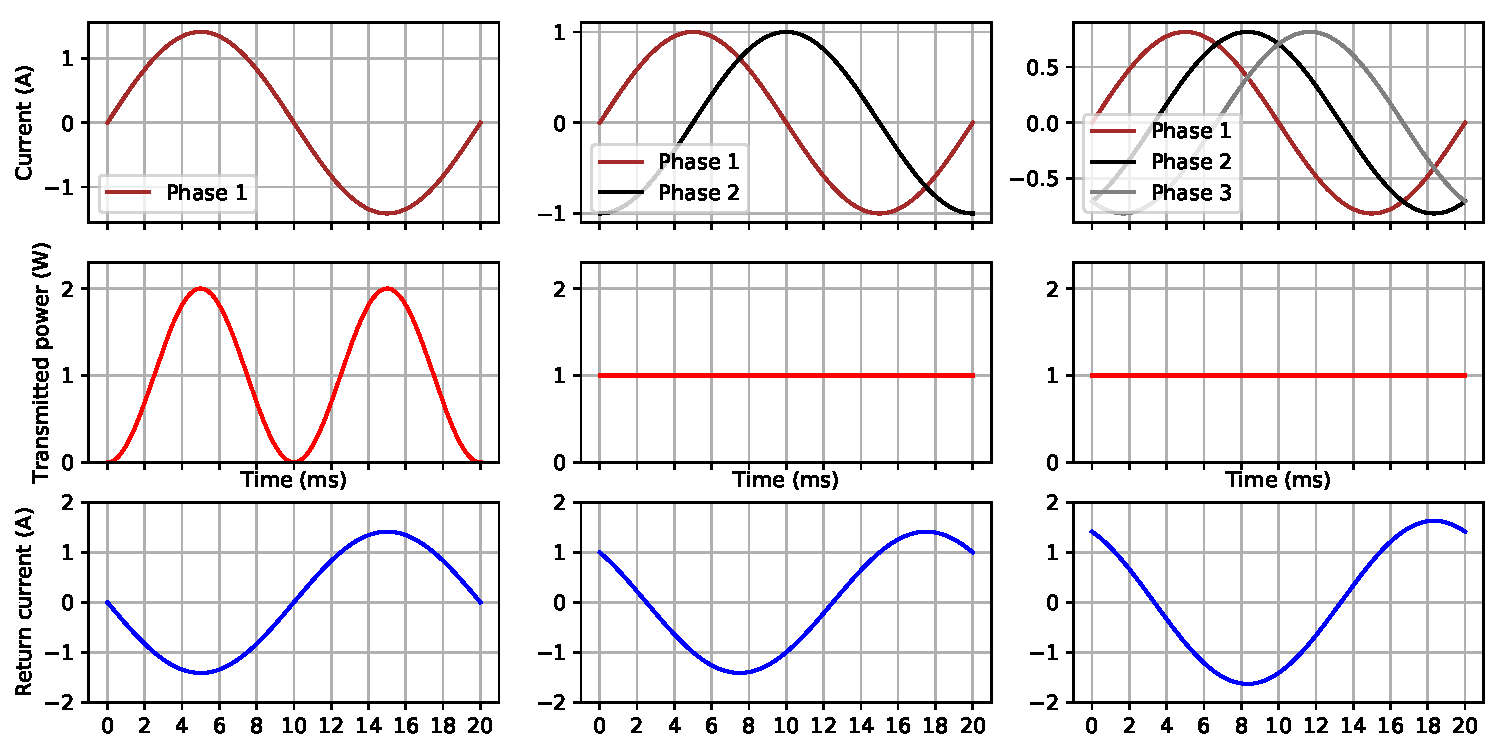
\includegraphics[width=\textwidth]{img/3phaseshalf.pdf}
    \caption{Phases distributed along half a cycle.}\label{fig:threephasehalfcycle}
\end{subfigure}
\begin{subfigure}{\textwidth}
    \centering
    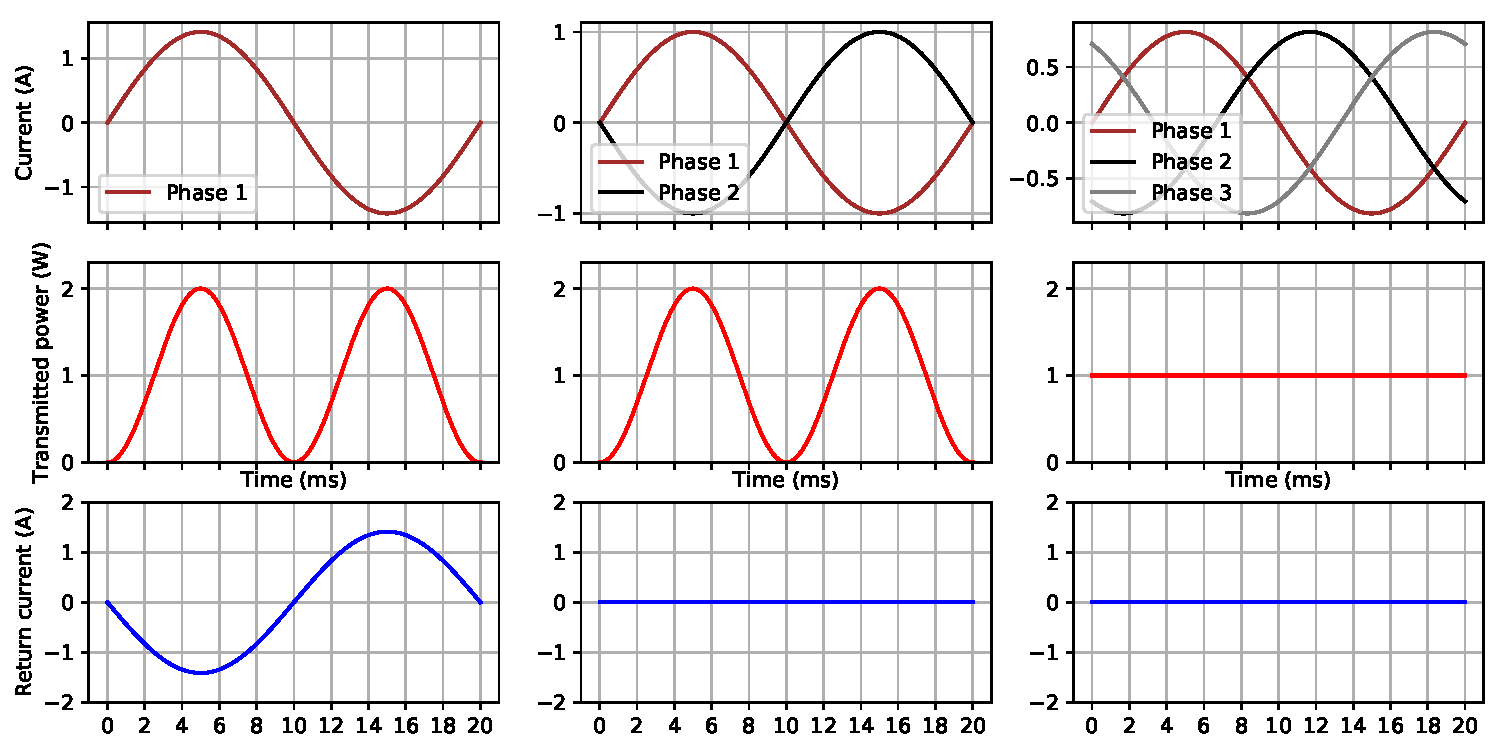
\includegraphics[width=\textwidth]{img/3phasesfull.pdf}
    \caption{Phases distributed along a full cycle.}\label{fig:threephasefullcycle}
\end{subfigure}
    \caption{Simulation of line current and transmitted power for one-phase, two-phase and three-phase transmission. The circuit consists of one, two or three identical resistors ($1 \, \si{\ohm}$), connected using the Wye configuration. Line voltage is chosen to produce a fixed amount of power ($1 \, \si{\watt}$). }
\end{figure}

Figure \ref{fig:threephasehalfcycle} shows one cycle of single-phase, two-phase and three-phase current, and the total amount of power transmitted by the phases. Here we see that the total amount of power is constant when more than one phase is used. So why not use two phases, instead of three?

Because electricity needs to flow in a \emph{closed circuit}, each phase needs \emph{two wires} to transmit its power; this second wire is called the \emph{return} wire. When we have more than one phase, their circuits are distinct, and we can combine their return wires into a single return wire for all phases.\footnote{using the Wye configuration described previously} This means that one-phase, two-phase and three-phase transmission requires two, three and four wires, respectively: one additional wire is the common return wire.

This return current is generally greater than each of the individual phase currents (see Figure \ref{fig:threephasehalfcycle}). However, when three-phase transmission is used with relative phase angles $0\si{\degree}$, $120\si{\degree}$ and $240\si{\degree}$, the return current is zero. This means that the return wire can be thinner (\ie cheaper), or it can be omitted completely.\footnote{In high-voltage transmission lines, one can often see a fourth (or seventh, or tenth), thinner wire: this is the return wire. This wire accounts for small imbalances in the load connected to each phase, which cause a non-zero return current. In some (older) medium-voltage lines, there is no return wire. In this case, the Delta configuration is often used: loads are connected to two of the three phases.} It is for these two reasons (constant power and no return current) that three-phase AC is used almost everywhere. 

When looking at AC transmission systems, you will often find three identical copies of the same component. For example, high-voltage AC transmission lines always have three, six or nine wires, which are identical in material, thickness and length. 

\subsubsection{Single-line approximation}
There are a number of reasons to build transmission systems this way. One benefit of having three copies of the exact same network is that they will behave the same way, saving grid operators up to two thirds of potential headaches!

As a result, it is very common to model the grid as a single-line network (with a global, zero-impedance ground). Because of the homogeneity of the transmission system, there are only some special cases where considering the three phases separately is necessary. See \cite{Kirtley2010} for a more detailed account.

\subsection{Line failures}\label{sec:linefailures}
When a transmission line stops transmitting power, we speak of a \define{line failure}. In most cases, a line failure is not caused by a broken or molten wire, but by a disconnection at one of its ends, as a safety measure. 
Some line failures are caused by a \define{fault}, or \emph{power surge} a sudden abnormal peak in current, caused by anomalies like fallen trees or lightning strikes. A high current is detected by \emph{circuit breakers}\index{circuit breaker}, which then automatically breaks its connection. A household fuse is an example of a circuit breaker, although modern circuit breakers use a mechanical switch. (These can be reset, instead of requiring a replacement fuse.) In high-voltage systems, circuit breakers can be quite advanced, sometimes using pressurised gas or oil to prevent arcing inside the switch.

Another type of line failure, the one most relevant to this thesis, is an \define{overload}. All transmission lines have a \define{thermal limit}: a maximum current that the line can sustain without risking overheating, causing sagging or even melting of transmission cables. To prevent these dangerous scenarios, transmission lines automatically disconnect when the current exceeds the predetermined \define{line threshold}.\footnote{The line limit of very long transmission is determined by the \emph{stability limit}, not the thermal limit. Using these lines beyond their stability limit causes the \emph{stable equilibrium} between the generators at its endpoints to be lost. See \cite{VonMeier2006}.}

It is important to note that grid operators cannot control the amount of current - and therefore - power that flows through a transmission line: grid operators can only connect or disconnect the line from the grid. The impedance of a wire does not act as a \emph{bottleneck} (like a small-diameter pipe would do in an irrigation network). From Ohm's law ($\phym{ZI=V}$), one could mistakenly conclude that the amount of current passing through a transmission line is inversely proportional to its resistance. However, the electric potential ($\phym{V}$) in this equation is \emph{not} the potential between the wire and the ground (\eg $220\,\si{\kilo\volt}$), but rather the potential difference between the two ends of the wire (which is not zero!). This difference (known as \define{line drop}) is quite low, compared to the potential between one of the ends and the ground ($220\,\si{\kilo\volt}$ transmission lines usually have a $1\si{\percent}$ line drop). The amount of current carried by a wire is dominated by the current being 'generated' and 'used' at its ends.
%
%\towrite{dynamic rating: modern transmission lines will allow a current beyond its threshold for a short while, and will have different ratings for different weather conditions}

\section{Grid security}\label{sec:powerflow}
Historically, failures of transmission network have had dramatic effects. The effects of such outages are even visible from space, since almost every light source depends on a functioning transmission network. 

Power outages can also be dangerous to human health. During the two-day blackout of Ontario and eight North-Eastern US states in 2003, almost 100 deaths were attributed to unavailable emergency services, stress, increased air pollution and the use of candles and backup generators.

%Luckily, TODO where a power-outage would be life-threatening, or has significant economic impact, often have backup generators in place.
%
%In modern hospitals, medical equipment often has a built-in battery to sustain relatively short power cuts. (When unplugged by accident, for example.) Hospitals also use two sets of power lines with independent protection: one for essential equipment, and one for computers, lights, phone chargers, et cetera.
%
%It should come as no surprise that the transmission network requires constant monitoring to ensure that it is working properly. 
%
When the first power grids were built, grid security was ensured by \emph{redundancy}. Transmission lines were designed to carry currents much greater than predicted. One of the criteria for building a network was \emph{N-1 redundancy}: the network should remain operational after the failure of \emph{any} line. In graph theory, this is equivalent to building a 2-edge-connected graph.

Nowadays, the capacity of power grids is being pushed to its limits. The main reason is that it is \emph{economically beneficial} to do so: most electricity networks have become \emph{privatised} since they were built, and are being used and upgraded in a way that minimises costs. A second reason is an increase in renewable generation, which requires the grid to be used in a way different from its design. This has led to ``more situations in which transmission lines are loaded close to their thermal limits.'' \citep{Ronellenfitsch2017}

There are many mechanisms in place that ensure grid security. For example, a grid operator has a \emph{load shedding scheme}: a predefined order of loads that will be cut off from the network when needed. The most important tool to maintain grid security is \emph{load profiling} (\ie predicting future load), combined with control over generation: the grid operator gets the final say in deciding which generators will be used at what time. We will discuss this decision-making process in Section \ref{sec:energymarket}.

Given the net amount of power injected at each node of the transmission network, the current that will flow through each line is determined by physics. We use a \emph{Power Flow} (PF) algorithm to calculate these currents, which we can use to check whether no line current exceeds its threshold. We will study the Power Flow equations in Chapter \ref{chap:model}.

\subsection{Power islanding}
Because nodes often house both loads and generators, the disconnection of a single node, or of a subset of nodes, does not always lead to a power outage, since local power generation might be sufficient to serve the load. This situation, where a subsection of the transmission network still operates after being disconnected, is called a \emph{power island}. 

Since the power island and the remaining network have been operating independently of each other, it is likely that their AC phase angles no longer line up.\footnote{This misalignment likely occurs right after the disconnection, when the total generation in the power island is substantially higher or lower than the total load. Until this mismatch has settled, the AC frequency will be higher or lower, respectively, than the target frequency (say, $50\,\si{\hertz}$).}
Unless this phase drift is corrected for (by temporarily increasing or decreasing the AC frequency on either side), the power island cannot be reconnected, since this phase drift likely exceeds the power angle limit of a new transmission line. 
%
%\towrite{historic note, slack bus, distributive slack, DC approximation, optimal power flow}

\section{The energy market}\label{sec:energymarket}
Modern power grids play the role of a competitive economic market. There are many possible ways to supply everyone with power, because there is more \emph{installed capacity} than there is demand. As a result, generation shares are largely determined by \emph{bidding}. Different generation technologies (gas, wind, etc.) form a \emph{stacking order}: in general, wind energy will always be cheaper than coal. Yet, it is not uncommon for renewable, cheap energy sources to be \emph{curtailed}, in favour of more expensive, possibly non-renewable energy sources. One of the reasons for grid operators to do so, is to protect vulnerable lines from overloading. 

\emph{In this section, we will describe a \textbf{very simplified} version of the energy market, to illustrate how grid operators ensure \emph{grid security} while minimising costs.}

Every hour, all parties involved in the generation and transmission of power come together, to decide \emph{what the configuration during the following hour will be}. For the sake of simplicity, we will assume that each power plant (renewable or non-renewable) is owned by its own company, and that the entire transmission network is owned by a single grid operator.

\subsection*{Phase one: offering prices}
First, all generators offer to supply energy during the coming hour \emph{for a certain price per kWh}. Generally, company A, which owns a wind farm, will offer their energy for a lower price than company B, which owns a coal plant. The price offered by company A is lower because a wind farm has zero \define{marginal cost} - the cost of generating an additional unit of electricity, once the turbine has been built. No fuel or labour is needed to generate power using a wind turbine, it simply needs to not be turned off.

Besides marginal cost, there are two more factors that influence the offered price:
\begin{itemize}[itemsep=0em]
    \item Company A needs to pay back their initial investment, which increases the offered price.
    \item Government subsidies, which promote the use of low-carbon energy, reduce the offered price.
\end{itemize}
In general, one can assume that the price offered for renewable energy is close to zero. In some cases, the subsidies are greater than all other costs, and energy is offered for a \emph{negative price}. This has the counter-intuitive effect that a grid operator actually \emph{earns money} by buying electricity from that company.

Energy from company B is generally more expensive, since it has a marginal cost (price of coal, labour wages, and so on), on top of paying back the investment.\footnote{In some cases, coal plants offer their electricity for a lower, or even negative, price, to avoid power off the plant. With the exception of open-cycle gas turbines, turning on non-renewable energy plants is expensive, and might take several hours. It might be cheaper for company B to offer their energy for free for one hour than to turn off the plant.}

Besides offering their marginal price, generators will also state their \define{generation capacity}.\footnote{This use of the word \emph{capacity} is entirely different from the \emph{capacity} of a capacitor, used in electrical engineering.} For some generators, this will always be the same amount. For a solar park, however, this capacity varies drastically, and needs to be estimated.

\subsubsection*{Marginal emissions}
The \emph{environmental cost} of a generator is mostly dependent on its energy source. In the context of global warming, we are interested in the amount of \emph{radiative forcing caused by greenhouse gases} that are emitted to generate energy, which is usually expressed as \emph{equivalent kilograms of CO$_2$}. Just like the financial cost, we usually speak of the \emph{marginal} emission of a certain generator: $\si{\kilo\gram}\text{CO}_2\text{eq} / \si{\kilo\watt\hour}$. See \cite{IPCCWG3AR5} for a summary of marginal emissions of each energy source.

\subsection*{Phase two: grid operator}
Now that all generators have offered a price, the grid operator needs to decide where to buy its energy from. Grid operators have a fairly good estimate for the load (energy demand) during the coming hour, based on the current load, historical load series, weather forecasts, sporting events, television programme schedules, and so on. Such a model is called a \define{load profile}.

By design, the total generation capacity is much greater than the expected load,\footnote{to account for so-called \emph{incident load}: the maximum amount of expected load. This amount is only likely to occur after a short blackout, when all consumer devices turn on simultaneously, and start cooling fridges and heating houses.} so running every generator at full capacity would be problematic.
As a grid operator, we need to tell each generator at what percentage of their capacity they should operate.

A complete set of generator instructions, called a \define{configuration}, might look something like Table \ref{tab:sampleconfiguration}. Note that generators could be told to operate at 0\% of their capacity, which is equivalent to powering off the generator completely.

\begin{table}[t]
    \centering
\begin{tabular}{l@{\hskip 2em}l@{\hskip 2em}l}
\toprule
    \multicolumn{3}{c}{\texttt{%\textbf{Configuration}, 
    15 March 2019, 11:00-12:00}}\\[.5em]
    \emph{generator} & \emph{offered price} & \emph{requested output} \\
\midrule
    \texttt{Sally's Solar Park} & \texttt{\hphantom{xx}4 \euro/MWh}  & \texttt{ 115 MW \emph{/ \hphantom{x}115 MW}} \\
    \texttt{Chris's Coal Plant} & \texttt{122 \euro/MWh}  & \texttt{\hphantom{xxx}0 MW \emph{/\hphantom{xx}240 MW}} \\
    \texttt{Nellie's Nuclear Plant} & \texttt{\hphantom{x}45 \euro/MWh}  & \texttt{1387 MW \emph{/ 2500 MW}} \\
    \texttt{Steven's Solar Park} & \texttt{\hphantom{x}-2 \euro/MWh}  & \texttt{\hphantom{xx}23 MW \emph{/ \hphantom{xx}23 MW}} \\
    $\qquad\vdots$ & \texttt{\hphantom{xx}}$\vdots$  & \texttt{\hphantom{xxx}}$\vdots$ \\
\bottomrule
\end{tabular}
    \caption{A small section of a fictional configuration.}
    \label{tab:sampleconfiguration}
\end{table}


Some configurations are more expensive than others, and some will result in more greenhouse gas emissions than others. Perhaps surprisingly, most configurations are not even \emph{admissible}: using them would cause some transmission lines to be overloaded, which could even result in a blackout.

More precisely, a configuration is called \define{ready to deploy} if it satisfies the following three conditions:
\begin{itemize}[labelwidth =\widthof{\emph{admissibleasdf}}, leftmargin = !]
    \item[\emph{possible}\index{configuration!possible}:] For each generator, the power output dictated by a configuration must be a non-negative number, no greater than the maximum capacity of the generator.
    \item[\emph{balanced}\index{configuration!balanced}:] When the dictated configuration is applied, total generation must equal total load, together with line losses.\footnote{Of course, the total load is not perfectly constant for one hour. To accommodate for this, the grid operator designates a single \define{load following} generator, which will vary its output continually to make sure that the total demand is met exactly. (This is equivalent to maintaining a constant AC frequency!) The bus that this generator is connected to is called the \define{slack bus} of the transmission network.}
    \item[\emph{admissible}\index{configuration!admissible}:] When the dictated configuration is applied, no line should be overloaded.
\end{itemize}

To determine whether a configuration is \emph{admissible}, the grid operator can simply \emph{calculate the line flows} that would be induced by that configuration, using a Power Flow (PF) algorithm, and check for any overloaded lines. Because power flow physics are quite well-understood, these results are accurate.

\subsection{Optimum Power Flow}
We can easily find a configuration that is both {possible} and {balanced}. First, set all generators to maximum capacity. We now have a \emph{possible} configuration. By design, the total generation of this configuration is much greater than the total load. By scaling the output of all generators with the same factor $0 \leq \lambda \leq 1$, the configuration remains \emph{possible}, and by the intermediate value theorem, a $\lambda$ exists such that the configuration is \emph{balanced}.

When trying out different \emph{possible}, \emph{balanced} configurations randomly, we will find that almost all of them are inadmissible; the subset of admissible configurations is actually quite small, and finding \emph{any} ready-to-deploy configuration is a lot of work.

Once a {ready-to-deploy} configuration has been found, the grid operator now wants to minimise economic and environmental cost. Given this initial configuration, the associated cost can be calculated, since all generators have offered their price, and their environmental impacts are known. 
This {ready-to-deploy} configuration is not unique, and by varying the configuration only slightly, the configuration remains ready to deploy.\footnote{As we will later learn, the function that maps a configuration to the vector of line flows that it induces is \emph{continuous}. The set of vectors where each line flow is $<100\si{\percent}$ is an \emph{open} box, and so its inverse image (the set of configurations that are ready to deploy) is also open.}
By doing so, we might be able to reduce the (environmental) cost! By repeating this process, a local minimum can be found. 

The problem of
\begin{gather*}
    \textit{finding a ready-to-deploy configuration} \\
    \textit{that minimises the associated cost} \nonumber
\end{gather*}
is called the \define{Optimum Power Flow (OPF)} problem. 

Even with modern-day computers, solving this problem is a difficult task indeed, and is often simplified by making a slight modification to our process. Instead of using the Power Flow (PF) algorithm to check a configuration's admissibility, we use the so-called \define{Linearised Power Flow (LPF)} algorithm to check linear admissibility. This linearised version can be computed much more quickly, with only a small loss in accuracy. We will derive the equations describing these two algorithms in Chapter \ref{chap:model}, and compare their results.

With our slight modification, we restate our problem as:
\begin{equation*}
    \begin{array}{ll@{}}
\text{minimise}  & \textit{associated cost} \\
\text{subject to}& \textit{possibility} \\
\text{and}& \textit{balance} \\
\text{and}& \textit{linear admissibility}
\end{array}
\end{equation*}
which is known as the \define{Linear Optimum Power Flow (LOPF)} problem. As suggested by the notation, this optimisation problem falls in the more general class of problems solvable using \emph{linear programming}. First studied by  Fourier in 1827, the field has seen many developments, most notably the \emph{simplex} solution method developed by G. Dantzig in 1947.\footnote{For the \emph{simplex method}, see \cite{Matousek2007} .}
Nowadays, several high-performance linear programming solvers have been created, including the open source \texttt{GNU Linear Programming Kit}, which was used in this project.

Using the LPF algorithm introduces a small error. For this reason, the \emph{admissibility} bounds are often scaled down by a contingency factor,\footnote{A contingency factor of $0.7$ is common.} creating a margin of error for line flows.
\end{document}